
\textbf{Appendix}

\begin{figure}[H]
    \centering
    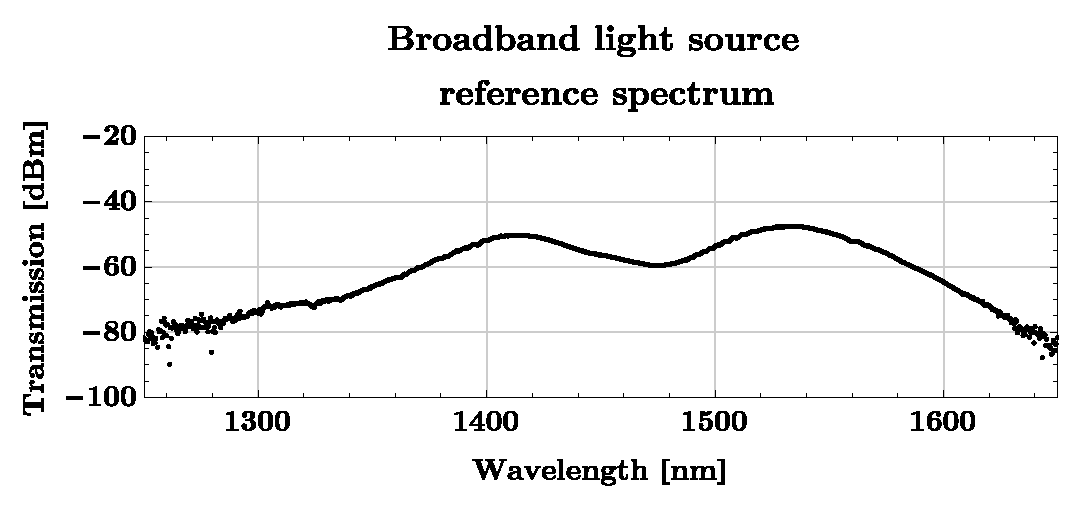
\includegraphics[width=0.7\textwidth]
    {fig/appendixrefplots/broadbandref.eps}
\vspace{-2mm}
    \caption{A typical reference spectrum for the broadband light source.}
    \label{fig:broadbandref}
\end{figure}

\vspace{-1.5cm}
\pagenumbering{gobble}

\begin{figure}[H]
    \centering
    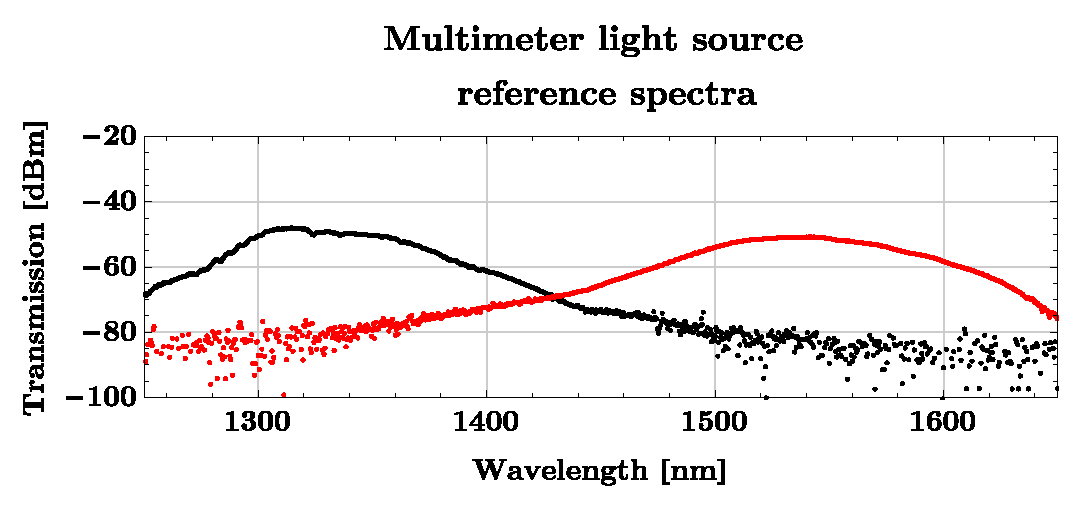
\includegraphics[width=0.7\textwidth]
    {fig/appendixrefplots/multimeterref.eps}
\vspace{-2mm}
    \caption{Typical reference spectra for the multimeter light source.}
    \label{fig:multimeterref}
\end{figure}

\vspace{-1.5cm}
\begin{figure}[H]
    \centering
    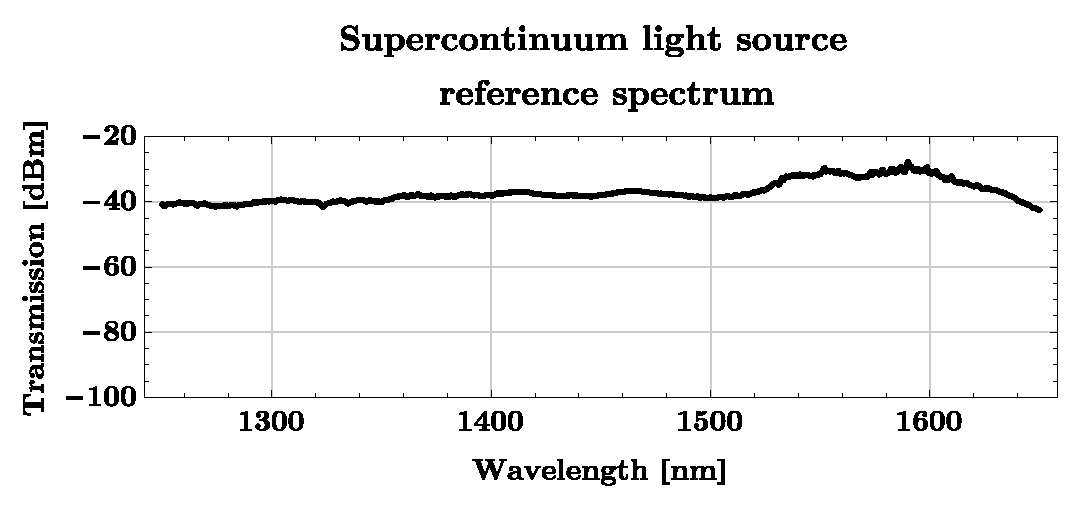
\includegraphics[width=0.7\textwidth]
    {fig/appendixrefplots/superKref.eps}
\vspace{-2mm}
    \caption{A typical reference spectrum for the supercontinuum light source.}
    \label{fig:superKref}
\end{figure}

\vspace{-1.5cm}
\begin{figure}[H]
    \centering
    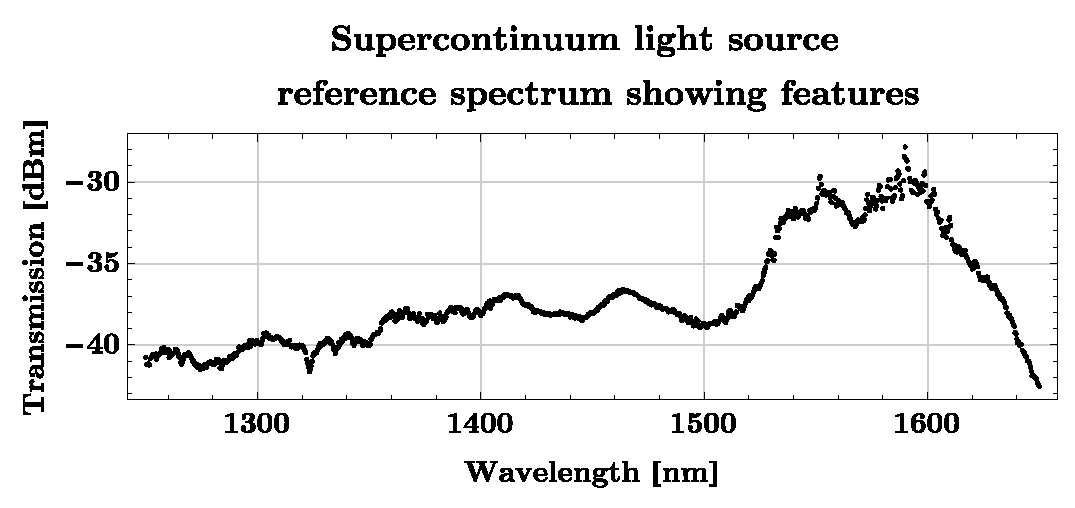
\includegraphics[width=0.7\textwidth]
    {fig/appendixrefplots/superKrefzoom.eps}
\vspace{-2mm}
    \caption{A typical reference spectrum for the supercontinuum light source showing the graph's features.}
    \label{fig:superKref}
\end{figure}


\begin{figure}[H]
    \centering
    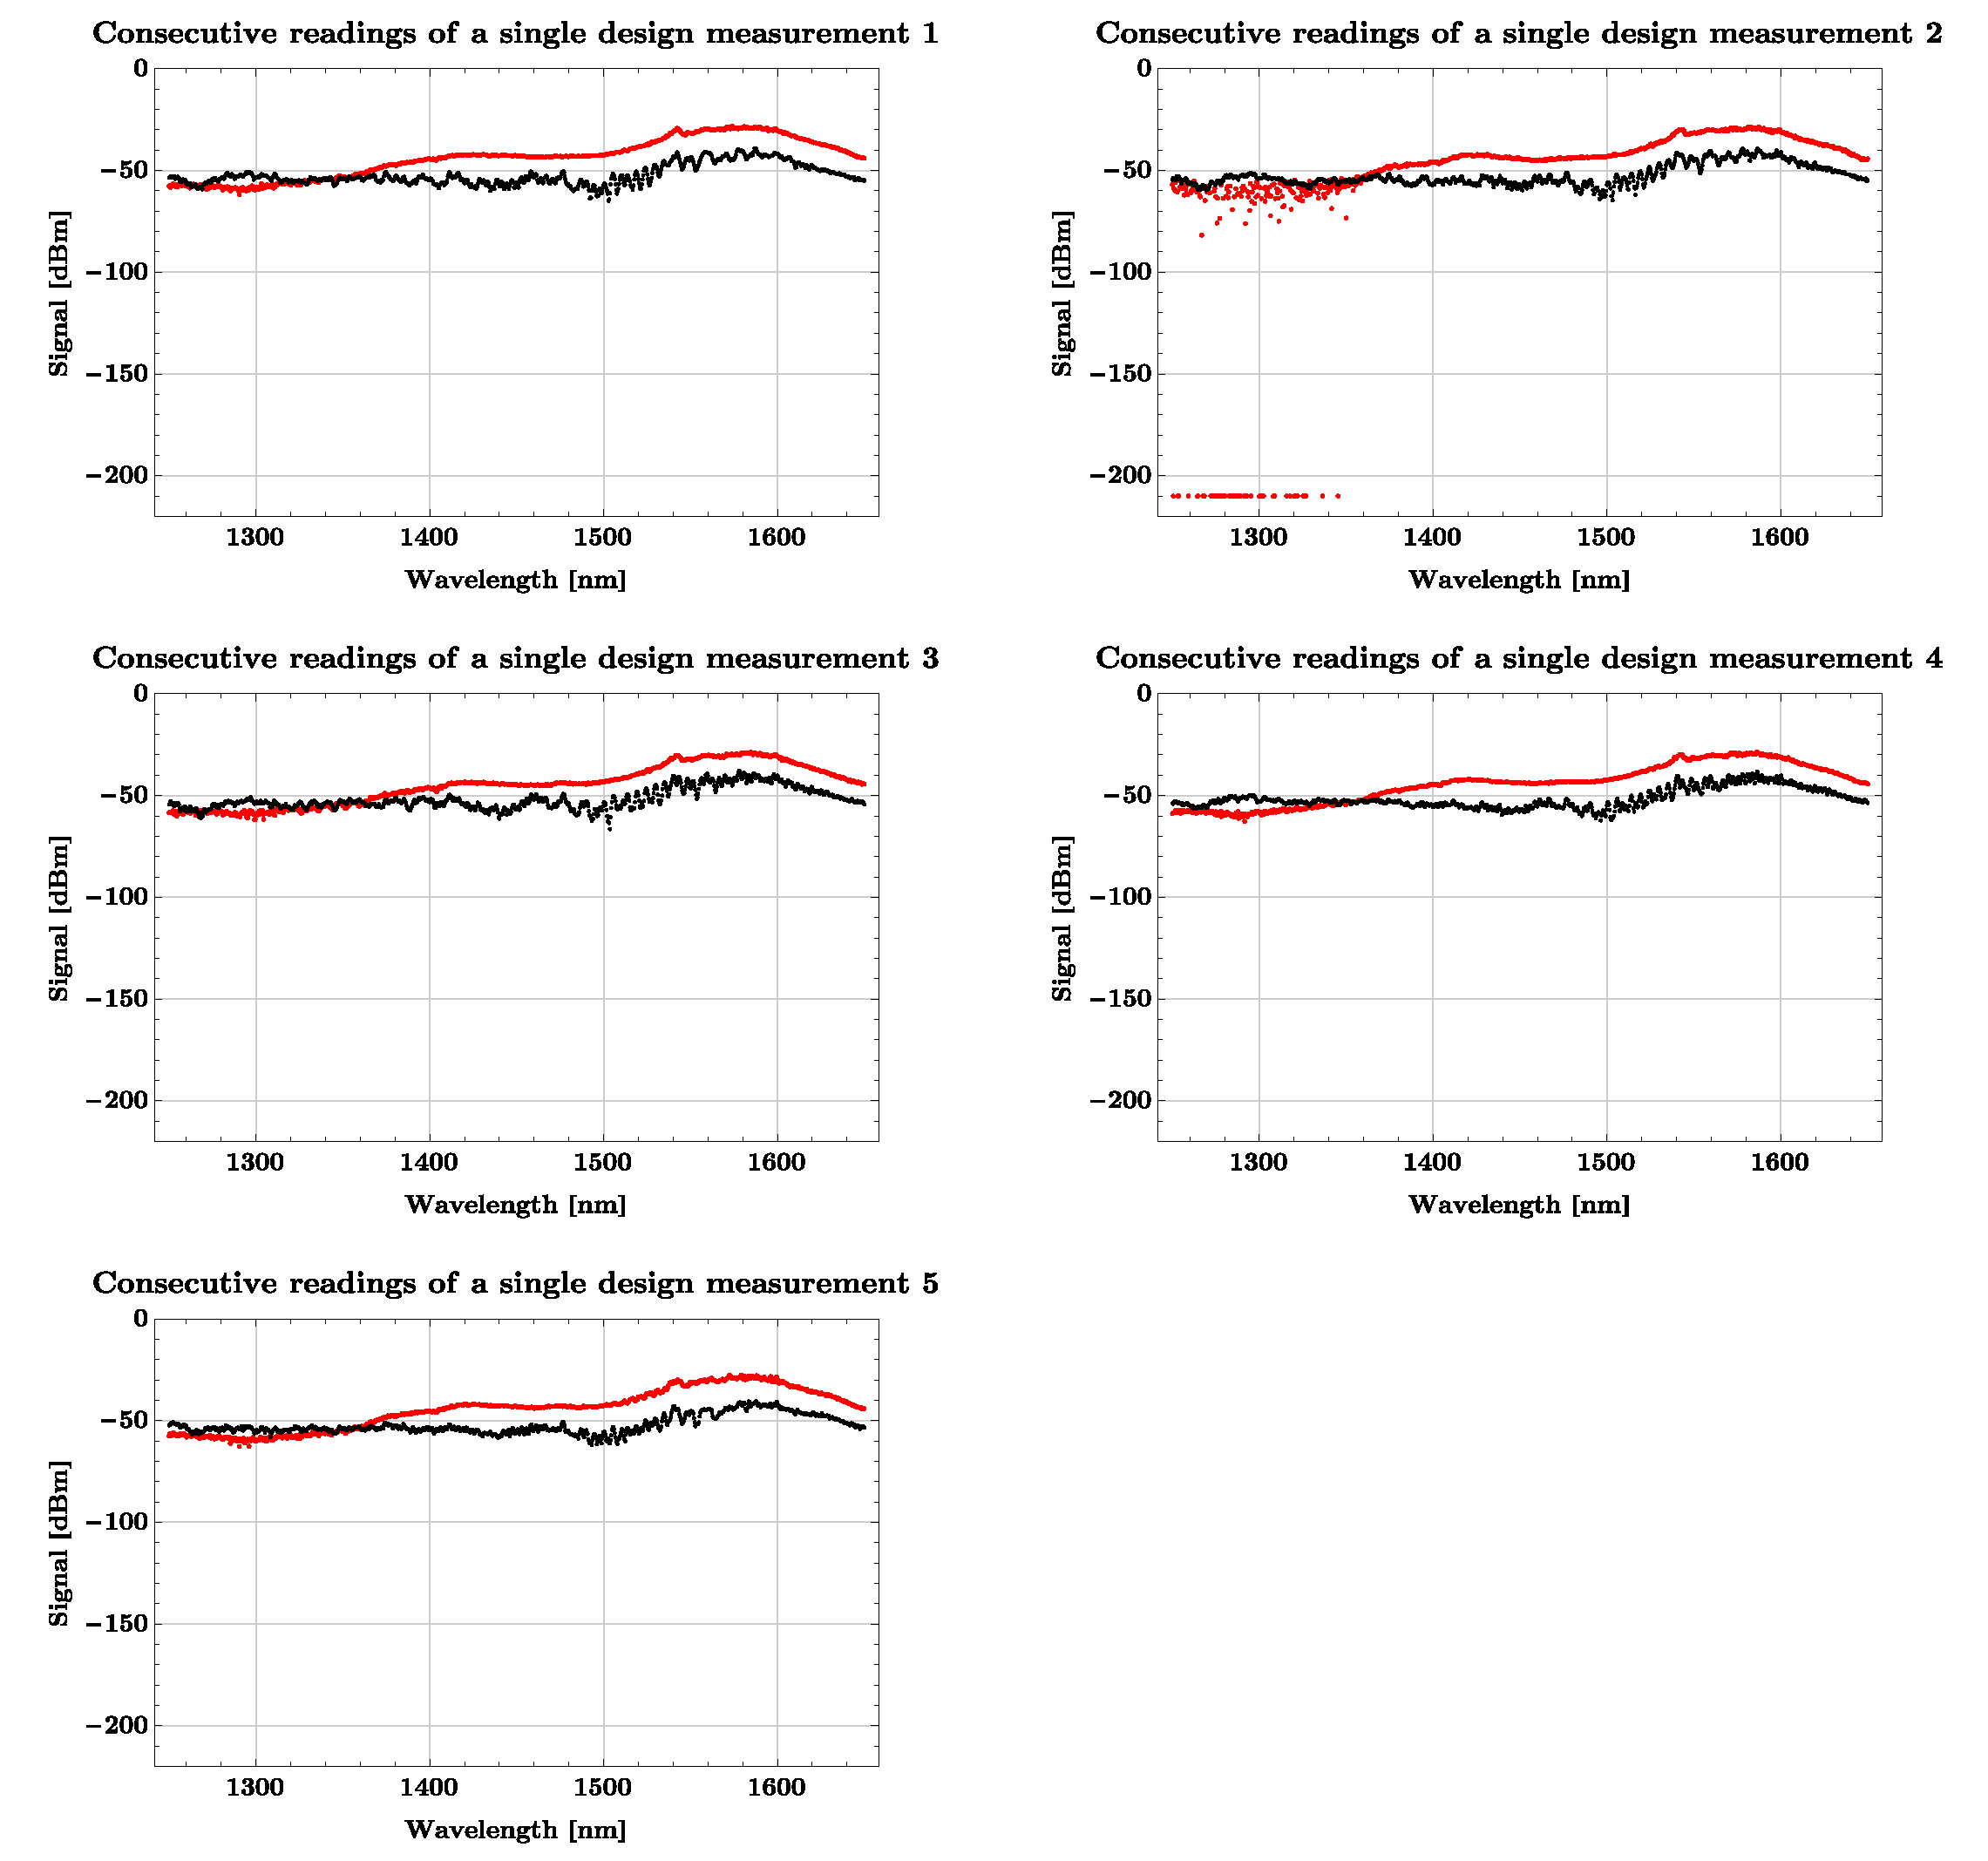
\includegraphics[width=1\textwidth]{fig/appendixrefplots/SignalPlots.eps}
    \caption{The sample of five measurements for consecutive readings on a single design (box 40 nm) with one sample having intensities below the sensitivity of the OSA, as seen on measurement 2.}
    \label{fig:ConsecutiveFiveBox40}
\end{figure}


